\chapter{Introduction}
\label{ch:intro}

\section{Memory errors}

Developing software is difficult. Developing software that is bug-free is all but impossible. ``Low-level'' programming languages such as C and C++ offer a great deal of control to the programmer, allowing them to write small and efficient computer programs. However, they also require the programmer to take a great deal of care with their development: the same level of control that allows extremely efficient software to be built also places a large burden on the developer, as making mistakes has steeper consequences than in higher-level, safer programming languages such as Java or C\#. (Indeed, this is one of the primary motivators for working in high-level languages.)

Typically, low-level programming languages require the programmers to manage memory manually, while higher-level languages generally include a garbage collector (GC) that frees the programmer from this burden. Managing memory manually means that objects whose lifetime is dynamic (not tied to a particular program scope) have to be \emph{allocated} as well as \emph{deallocated} (freed) explicitly.

In C, such memory allocation typically occurs using the \lstinline!malloc()! or \lstinline!calloc()! functions. These allocate a region inside the \emph{heap memory} of the application, reserving it for use, and returning a pointer (typically, an untyped \lstinline!void *!) to it. On the x86 and x86-64 architectures, which we will mainly concern ourselves with in this thesis, a pointer is just a linear memory address: a number representing the index of the first byte of the pointed region in the main memory. This makes pointer arithmetic, such as accessing \lstinline!numbers[4]! in a \lstinline!int *numbers! very easy and efficient to perform: just load \lstinline!sizeof(int)! bytes from the memory address \lstinline!(uintptr_t)numbers + 4 * sizeof(int)!. Conversely, after we are done with using a given memory region, we can and should deallocate it using the \lstinline!free()! function. This marks the memory region as no longer in use, and potentially reusable -- a characteristic that forms the basis of this thesis.

In C++, memory allocation typically happens using the \lstinline!new! or \lstinline!new[]! operators, and deallocation using the \lstinline!delete! or \lstinline!delete[]! operators. However, these behave exactly like \lstinline!malloc()! and \lstinline!free()! used in C in all ways that are important from a memory management point of view. I should note that in modern C++, the use of such memory management is discouraged and generally unnecessary since \emph{smart pointers} -- wrappers around pointers that automate the lifecycle management of the pointed memory region, conceptually similarly to a garbage collector -- were introduced. However, a lot of applications are still being developed and maintained that do not make use of such features.

Making mistakes with manual memory management is very easy. Allocating but not freeing a memory region even after it is no longer used is called a \emph{memory leak} and it increases the memory usage of the application, often in an unbounded manner, potentially until a crash occurs due to insufficient memory. Attempting to deallocate an object twice -- \emph{double free} -- causes the memory allocator to attempt to access accounting data stored typically alongside the user data in the since-freed region, often leading to seemingly nonsensical behaviour or a crash, given that the region may have been re-used. Accessing an offset that falls outside the memory region reserved for the object -- \emph{out-of-bounds access}, sometimes also called \emph{buffer overflow} or \emph{buffer underflow} -- can lead to reading unexpected data or overwriting an unrelated object, again often causing hard-to-understand bugs and crashes. One example for this would be attempting to write to \lstinline!numbers[5]! when only enough space to hold 5 elements was allocated, e.g.\ using \lstinline!int *numbers  = malloc(5 * sizeof(int))! (recall that in C and related languages, indexes start at 0, so the first item is located at index 0, the second at index 1, and so on). Finally, accessing a memory region that has been deallocated -- \emph{use after free} -- is similarly problematic. This generally occurs when a pointer is not cleaned up along with the object it referenced, leaving it dangling; often also called a \emph{dangling pointer}~\cite{dangling-ptr-smashing-webpdf}.

Besides the instability and general mayhem that such memory errors routinely cause, they can also leave the application vulnerable to attacks, for instance by enabling unchecked reads or writes to sensitive data, sometimes even allowing an attacker to hijack the control flow of the application, execute almost arbitrary instructions, and in essence take over the application.

It should be clear by now why modern, ``high-level'' programming languages restrict or completely prohibit the direct use of pointers, often by making it impossible and unnecessary to manage memory manually. In such languages, the programmer can perform allocations only by creating objects (preventing another class of bugs relating to the use of uninitialized memory), and leaving their deallocation to the runtime environment, commonly its component called the garbage collector (GC). The GC will periodically analyse the memory of the application, and upon finding objects that are no longer referenced, marks them for reclaiming, and eventually deallocating them automatically. This, of course, comes at a cost in performance, often one that is unpredictable as the GC is controlled by the runtime environment as opposed to the user code. (It is worth noting that this scheme does not protect against all possibilities of memory errors; for instance, leaks are still both possible and common.)

A notable exception is the Rust programming language, which, while does allow pointers, heavily restricts how they can be used, preventing any code that could potentially be unsafe. It does so using static (compile-time) checking using their so-called \emph{borrow checker}. However, realizing that in doing so it also disallows some valid uses of pointers, it also provides an escape hatch, allowing code sections to be marked as \emph{unsafe} and go unchecked. (For example, it is not possible to implement a linked list in safe Rust, and even the built-in \lstinline!vec! type is written using unsafe code.) Another programming language that follows a similar pattern is C\#: normally used as a high-level, managed language employing a GC, it also allows pointers to be used directly in code marked as unsafe~\footnote{Usage of raw pointers in an otherwise managed environment comes with caveats; for instance, the memory is often compacted after GC passes with the surviving objects moved next to each other to reduce fragmentation. Such relocation is not possible if there are raw pointers in play; therefore, programmers are required to mark the pointers they use as \emph{pinned} using the \lstinline!fixed()! construct.}.

Still, applications written in languages like C or (older) C++ with no safe alternatives to pointers have been written and are being maintained, and these applications remain affected by memory errors. Significant amount of research has been and continues to be conducted in this topic, as such applications are often high-value targets for attackers: operating system kernels, device drivers, web servers, anti-virus programs are commonly developed using these technologies.

This thesis is focused specifically on dangling pointer errors, a class of memory issues defending against which has traditionally been difficult and inefficient.

\section{Dangling pointers}

A pointer is said to be \emph{dangling} when it outlives the memory region it references. Dereferencing such a pointer will generally lead to unwanted, confusing behaviour.

In the very best-case scenario, the memory access fails, and the application is killed by the operating system kernel; for example on Unix systems by sending it a signal like \lstinline!SIGSEGV!, leading to the well-known ``Segmentation fault'' error and a groan from the programmer. This is useful (and often highly underrated by programmers), because it clearly indicates a bug, and the responsible memory address is readily available, greatly helping with debugging.

Unfortunately, in the majority of cases in practice, the memory access will not fail. The reason for this is that most modern architectures in widespread use (such as x86 and ARM) handle memory on the granularity of \emph{pages}, where a single page is usually 4096 bytes (4 kilobytes). From the point of view of the hardware and the kernel, a page is either in use or is not; pages are treated as a unit and are never split up. Of course, typical memory allocations tend to be significantly smaller than this, and it would be wasteful to dedicate an entire page of memory to just hold for instance 200 bytes of user data.

Therefore, all memory allocator implementations used in practice do split up pages, and will readily place two allocations on the same page, typically even directly next to each other (not counting any meta-data). After the deallocation of one of the objects, the page as a whole still remains in use, and so the hardware will not fault on subsequent accesses to it, regardless of the offset; see Figure~\ref{fig:mem_two_small_allocs}. Notably, even if a memory page holds no live objects, it is often still not returned to the system; the memory allocator retains it as an optimization, expecting more allocations in the future. (This is because the memory allocators being discussed run in user-space, so in order to gain access to memory pages to use, they have to perform a system call such as \lstinline|mmap()| or \lstinline|brk()|, which is costly.)

\begin{figure}
    \centering
    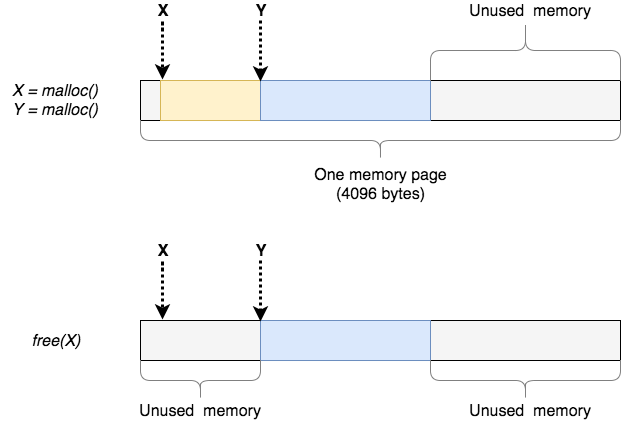
\includegraphics[width=\textwidth]{diagrams/dangling_pointer_basics.png}
    \caption{Memory layout of two small allocations. \emph{X} and \emph{Y} are pointers, referencing their corresponding memory regions. \emph{X} becomes dangling}
    \label{fig:mem_two_small_allocs}
\end{figure}

If a page is known to be unused by the hardware and kernel, then accessing it will trigger a page fault in the kernel, which will generally terminate the application, leading to the best-case scenario described earlier. This is a far more manageable problem than the alternative, because the error is clear, even if in practice it is often difficult to discover the underlying reason, given that time may have passed between the deallocation and attempted access, and so the code executing at the time of access may not have any relation to the code that was responsible for the deallocation. Furthermore, this scenario does not generally pose a security problem, as a crashed application is difficult to exploit. Therefore, I will generally ignore this scenario for the remainder of this thesis.

The effect of an unchecked access through a dangling pointer depends on whether or not the referenced memory region has been reused since the time of deallocation. If it has not, the data read often will still be valid, and execution may continue without anyone the wiser, masking the bug -- at least until a modification in the code or one of the libraries leads to a change in the memory allocation pattern. Otherwise, the dangling pointer will point inside another allocation, and the data read or overwritten will almost always be a source of unexpected behaviour: see Figure~\ref{fig:normal_malloc}.

\begin{figure}
	\centering
	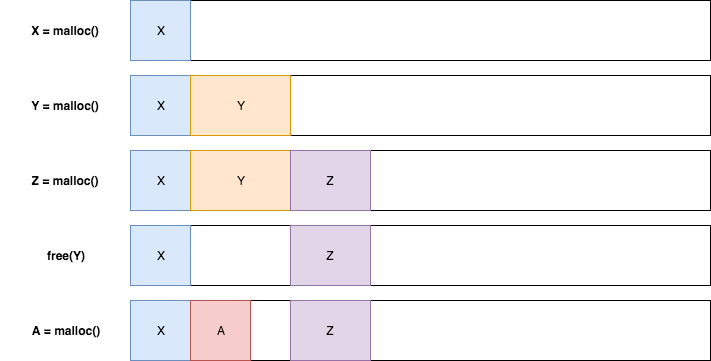
\includegraphics[width=\textwidth]{img/normal_malloc.png}
	\caption{(Simplified) Memory layout view when using traditional malloc(): memory is re-used}
	\label{fig:normal_malloc}
\end{figure}

One typical case is \emph{type confusion}: the value read or written will be treated as a different type than the value stored there. A string value can be for instance accessed as an integer, causing the characters that make up the string to be interpreted as bytes in an integer, essentially leading to the same behaviour as this code snippet:

\begin{lstlisting}
char *s = "foobar";
int i = *(int *)s;
\end{lstlisting}

This code compiles and runs successfully. What will be the value of \lstinline!i!? Of course, we are deep into undefined behaviour territory here, meaning that the programming language promises nothing. In practice, on x86-64 architectures where the \lstinline!int! C type is 4 bytes long (\lstinline!sizeof(int) == 4!), the result will typically be \texttt{1651470182}, or \texttt{0x626f6f66} in hexadecimal. This makes sense: the string \lstinline!"foobar"! (including the null terminator) is represented by the byte sequence \texttt{0x66 0x6f 0x6f 0x62 0x61 0x72 0x00}. Interpreting it as an \lstinline!int! means reading the first 4 bytes (\texttt{0x66 0x6f 0x6f 0x62}) and assembling it into a multi-byte integer according to the endianness of the processor. My laptop has an Intel CPU in it, which is little endian, meaning that the bytes of an integral type are stored as least significant byte first (this is \texttt{0x62}), followed by bytes of increasing significance; simply put, bytes are interpreted in ``reverse order''.

Of course, type confusion does not have to occur in order for invalid behaviour to occur. For instance, overwriting an Unix file descriptor with the number of characters in a text will typically result in an invalid file descriptor; or consider a buffer's length overwritten by the age of the user; or an integer representing the next free index in an array overwritten by the length of a file in bytes. Once memory corruption occurs, sanity flees.

\section{An example}

Let us look at a less trivial example. This is a simplistic codebase, written in C++ of an in-memory messaging system. Each \lstinline!User! has an inbox and outbox, \lstinline!Mailbox! objects, which wrap an \lstinline!std::vector<Message *>!. \lstinline!Message! objects are allocated on the heap, referenced by plain pointers, allowing the sender and recipient mailboxes to just both retain a pointer to the same message -- a memory optimization. Each message object keeps track of who has deleted it, and when both the sender and receiver have done so, the message can be safely deallocated.

\begin{lstlisting}
struct Message {
	const std::string mContent;

	$bool mHasSenderDeleted = false;$
	$bool mHasRecipientDeleted = false;$

	explicit Message(std::string content)
		:   mContent{std::move(content)}
	{}

	void OnDeleted() {
		@if (mHasSenderDeleted && mHasRecipientDeleted)@
			@delete this;@
	}
};

struct Mailbox {
	std::vector<Message*> mMessages;

	void AddMessage(Message* msg) {
		mMessages.push_back(msg);
	}

	void DeleteMessage(Message* msg) {
		mMessages.erase(std::find(mMessages.begin(), mMessages.end(), msg));
		msg->OnDeleted();
	}
};

struct User {
	Mailbox mInbox;
	Mailbox mOutbox;

	void SendMessage(User& recipient, std::string content) {
		Message* msg = new Message{std::move(content)};

		mOutbox.AddMessage(msg);
		recipient.mInbox.AddMessage(msg);
	}

	void DeleteReceivedMessage(Message* msg) {
		`msg->mHasRecipientDeleted = true;`
		mInbox.DeleteMessage(msg);
	}

	void DeleteSentMessage(Message* msg) {
		`msg->mHasSenderDeleted = true;`
		mOutbox.DeleteMessage(msg);
	}
};
\end{lstlisting}

The noteworthy lines have been highlighted. While this design is error-prone, as we will see, it does work correctly and does not -- in its current form -- represent a vulnerability.

However, code evolves over time as bugs are fixed and new features are added, often by a different developer than the original authors. Sometimes these programmers understand the codebase less, or have less experience with programming or the technologies used, and can easily make mistakes. Especially with a language like C and C++, mistakes are extremely easy to make, and sometimes hard to notice, let alone debug.

Consider now that another programmer comes along and has to implement a feature to allow forwarding messages. His deadline is in an hour, perhaps there is a presentation scheduled with a big client, and this feature was simply forgotten about until now. This programmer adds a simple function as a quick hack to get message forwarding to work, and schedules some time for next month to revisit the feature and implement it properly. This function is added:

\begin{lstlisting}
struct User {
// ...

	void ForwardMessage(User& recipient, Message* msg) {
		// TODO: do this properly later
		recipient.mInbox.AddMessage(msg);
	}

// ...
};
\end{lstlisting}

He did not understand how the simplistic reference counting of the \lstinline!Message! objects work, and a quick test showed that this feature seems to work reasonably well. His attention was quickly drawn away by another tasks and this code will not be revisited for a while.

The problem shows itself when a message that was forwarded gets destroyed. While the code correctly ensures that the message is removed from the both the sender and the recipient's mailbox before it can be destroyed, but any potential forwardees were not taken into account. Consider now the following chain of events:

\begin{lstlisting}
Message* funnyMessage = bob.SendMessage(alice, "Hey, look at this funny gif: <image>");
bob.DeleteSentMessage(funnyMessage);

alice.SendMessage(cecile, "Haha, look at this funny gif!");
alice.ForwardMessage(cecile, funnyMessage);

alice.SendMessage(bob, "HAHA that's pretty awesome");
alice.DeleteReceivedMessage(funnyMessage);
\end{lstlisting}

Bob sends a message to Alice, who forwards it to Cecile. Both Bob and Alice delete the message, causing the object to be destroyed, while Cecile's inbox still retains a pointer to it: a dangling pointer! What will happen if Cecile looks at her inbox? The application will attempt to dereference the dangling pointer, with unpredictable results.

What if there is another message, containing some sensitive information, is sent directly afterwards, potentially between completely unrelated users?

\begin{lstlisting}
bob.SendMessage(daniel, "My PIN code is 6666");
\end{lstlisting}

Depending on the memory allocator, it is entirely possible that the memory referenced by \lstinline!funnyMessage! before is now reused for the new, secret message. In this case, Cecile's inbox now contains a message not intended for her, containing sensitive information.

\begin{lstlisting}
for (const Message* msg : cecile.mInbox.mMessages) {
	std::cerr << msg->mContent << "\n";
}
\end{lstlisting}

The following output is produced when compiled with a recent version of GCC (regardless of optimizations or other options) and run:

\begin{verbatim}
Haha, look at this funny gif!	
My PIN code is 6666
\end{verbatim}

This is an example of how dangling pointer errors can pose a security vulnerability, even without the active efforts of an attacker.

It is worth noting that using a correct implementation of reference-counting, such as with the standard \lstinline!std::shared_ptr! (since C++11), this problem could have been avoided. However, while smart pointers go a long way towards making dynamic memory safer and more convenient to use, they do have limitations even in the current C++ version (C++17 as of the time of writing). For instance, it is common to use plain pointers to represent a non-owning, optional reference to memory owned by another object, such as an \lstinline!std::unique_ptr!, enabling dangling pointer errors to occur.

\subsection{Dangling pointers and late binding in C++}

Dangling pointers are an even more severe vulnerability in C++ because it supports the object-oriented programming paradigm, and therefore allows programmers to define classes, virtual methods, and express inheritance. In order to support virtual methods being overridden in derived classes, the C++ compiler creates a data structure called a \texttt{vtable} for each class that contains virtual methods, whether defined in the class or inherited from a base class. This \texttt{vtable} is essentially a look-up table, containing function pointers to the class's own implementations of the virtual methods. Furthermore, an additional \texttt{vptr} pointer field is added to any objects of such classes, which points to the correct \texttt{vtable}. This pointer value persists even through derived-to-base casts, to allow the program to behave as expected. For instance:

\begin{lstlisting}
class Base {
public:
	virtual ~Base() = default;

	virtual std::string getTypeName() const {
		return "Base";
	}
};
\end{lstlisting}

This defines a class \texttt{Base} with a virtual method \lstinline!getTypeName()!, the default implementation of which returns the string \lstinline!"Base"!. Since the class contains virtual methods, the C++ compiler emits a \texttt{vtable} for it with 2 entries: one for the destructor, and one for \lstinline!getTypeName()!, both of them pointing to \lstinline!Base!'s own implementations. When we call the \lstinline!Base()! constructor and instantiate an object of the class, it will contain a hidden field (usually as the first field, placed before any user-defined ones): the \texttt{vptr} that points to Base's own \texttt{vtable}. (The destructor has to be virtual, otherwise objects may not be correctly destroyed.)

\begin{lstlisting}
class Derived : public Base {
	std::string getTypeName() const override {
		return "Derived";
	}
};
\end{lstlisting}

We have now defined a second class which inherits from \lstinline!Base! and overrides \lstinline!getTypeName()! with its own implementation, one that returns \lstinline!"Derived"!. (The compiler also automatically emits a trivial destructor that overrides the base class'.) The \texttt{vtable} emitted for \lstinline!Derived! has the same structure as that of \lstinline!Base!, but contains the addresses to \lstinline!Derived!'s virtual method implementations. Similarly, when a \lstinline!Derived! object is constructed, the object contains a \texttt{vptr} hidden field pointing to its \texttt{vtable}.

\begin{lstlisting}
void print(const Base& obj) {
	std::cout << obj.getTypeName() << '\n';
}

int main() {
	print(Base{}); // prints "Base"
	print(Derived{}); // prints "Derived"
	return 0;
}
\end{lstlisting}

Note how the global function \lstinline!print()! accepts a \lstinline!const Base&!: this function has no idea about any derived of \lstinline!Base!. Yet when it calls the \lstinline!getTypeName()! method on it, the actual function executed is different between the two calls. The reason is that when a virtual method is called, the C++ compiler will emit code that dereferences the \texttt{vptr} field, searches the referenced \texttt{vtable} for the entry corresponding to the method being called, and performs an indirect function call to the address contained in the entry. This is how late binding function calls are implemented in C++.

Now we know enough to understand why dangling pointers are particularly dangerous in applications written in C++: should the attacker be able to construct its own fake \texttt{vtable} in memory, as well as get the application to perform a virtual method call on an object whose \texttt{vptr} field it managed to overwrite with one pointing to the fake \texttt{vtable}, the attacker can hijack the control flow of the application. This can be tricky to do, as the \texttt{vptr} is typically at the same offset in all objects, which makes it more difficult to overwrite with attacker-controlled data.

It is also worth noting that although rare, objects of classes that inherit from multiple base classes (since C++ allows multiple inheritance) have multiple \texttt{vptr} fields at different offsets. This potentially makes the job of the attacker easier. Furthermore, access through dangling pointers are not the only way to perform such an attack: a buffer overflow or underflow vulnerability in the object can also enable the attacker to hijack the \texttt{vptr} field.

Defenses against such attacks do exist: examples include SafeDispatch~\cite{cpp-vptr-safedispatch}, work by Gawlik et al~\cite{cpp-vptr-gawlik}, or the research of Bounov et al~\cite{cpp-vptr-bounov}.